%************************************************
\chapter{Load Testing and Performance Measurement}
\label{ch:performance-load-testing}
%************************************************

\section{Introduction}

\marginpar{When doing a use case analysis at the beginning of a project, always add an actor named ``system administrator'', or ``IT Ops engineer''. This will require the team to also look at the system from the point of view of people who run the system. This will encourage discussions about systemic qualities like reliability, scalability and security. Also, remember that every use case can be annotated with quantitative constraints (e.g. max response time, min throughput, etc.)}

When creating a software product, the team has two consider two types of requirements:

\begin{itemize}
\item the \emph{functional requirements} specify \emph{what} the software should do. When doing a use case analysis, the team identifies the actors (the categories of users and external systems) which interact with the system. The team also enlists the features provided by the system and captures them as a list of use cases and scenarios.
\item The \emph{non-functional requirements} specify and quantify various qualities that the system should have. For instance, the team should assess the needs in terms of performance, scalability, availability, security, maintainability, manageability, etc. This is a critical part of the analysis, because it should drive the architecture of the system. Making a sound architectural decision is about making the right \emph{tradeoff} between the cost of a solution and its impact on non-functional requirements. For instance, availability is always \emph{somewhat} important. It is possible, but very complex and costly to build systems with a 99.999\% uptime. Therefore, the first task is to define what is the appropriate availability level for the system. The second task is to propose a technical design that is expected to reach that level. The third task, very important and often overlooked, is to actually measure if the specified level is reached by the system. This has to be done through experiments and measurement.
\end{itemize}

\marginpar{An application that works when one developer tests it manually may break when 100 users access it at the same time.}

In this chapter we take a look at a particular non-functional aspect: how does the application behave under load? We explain how to setup experiments to measure performance, in terms of response time and throughput. We also show that testing an application under load can sometimes uncover bugs, particularly those related to concurrency. We present Apache JMeter, an open source tool that supports these testing activities.

\section{Testing web applications with Apache JMeter}

In the early 2000s, performing load tests on a web application required the use of expensive commercial tools. Apache JMeter was one of the first projects to offer an open source alternative. It has continuously evolved over time and remains a popular tool. Simply stated, JMeter allows you to define test scenarios, which are essentially sequences of HTTP requests (e.g. send a request to the login page, then a request to the account page, then a request to the products list page, etc.). When the scenario is ready, JMeter can simulate a large number of virtual users and thereby generate a load on the system. Measures are collected during this process and  It is extensible and a number of plugins are available on the \href{jmeter-plugins.org}{https://jmeter-plugins.org/} website. We recommend to install some of these plugins (in particular the plugins in the Thread Groups category), because they really improve the standard distribution.

\subsection{Installation}

Installing JMeter is very simple. An archive is available on the \href{https://jmeter.apache.org/download_jmeter.cgi}{project website}. The procedure to install plugins is described \href{https://jmeter-plugins.org/install/Install/}{in the documentation}. Once installed, JMeter is launched with a shell script located in the \texttt{bin} package.

\marginpar{Use the JMeter GUI to design and validate your automated tests. Disable the GUI to preserve resources when generating the real load.}

The message displayed on the terminal, shown in Listing \ref{lst:jmeterWarning} is important. It makes it clear that JMeter should be used in two phases. During the test design phase, it is a good idea to use the \ac{GUI} mode and to build the test scenarios with the interactive interface. However, once the test plan is ready, JMeter should be used in non-interactive mode to generate the load. The reason is that resources on the client machine should be used with care: the client should not be the bottleneck when running the test. How much load can be generated by JMeter, in other words how many concurrent users can be simulated, is not a trivial question. A special section in the documentation gives a few recommendations. Experts have also written articles on the topic and they are very useful when running a proper benchmark.

\lstset{
	caption={Warning displayed when launching JMeter},
	label={lst:jmeterWarning}
}
\vspace{10pt}
\begin{minipage}{\linewidth}
\begin{lstlisting}[frame=single]
================================================================================
Don't use GUI mode for load testing !, only for Test creation and Test debugging.
For load testing, use NON GUI Mode:
   jmeter -n -t [jmx file] -l [results file] -e -o [Path to web report folder]
& increase Java Heap to meet your test requirements:
   Modify current env variable HEAP="-Xms1g -Xmx1g -XX:MaxMetaspaceSize=256m" in the jmeter batch file
Check : https://jmeter.apache.org/usermanual/best-practices.html
================================================================================
\end{lstlisting}
\end{minipage}

\subsection{Concepts}

JMeter is used to create \emph{test plans}. It is recommended to create different test plans for different parts or aspects of the application, to keep them small and manageable. A test plan is stored in a \texttt{.jmx} file and can loaded when running JMeter in non-interactive mode.

A test plan is a tree of elements and JMeter defines different types of elements:

\begin{itemize}
\item \emph{Thread Groups} are used to simuate virtual users. There are different types of Thread Groups and it is important to understand how they work in order to interpret the test results. 
\item \emph{Samplers} are used to generate individual requests. Initially, JMeter was used only to test web applications and provided an HTTP sampler. Today, it is possible to generate load for other protocols, such as FTP, LDAP, JDBC, JMS, etc.
\item \emph{Logic Controllers} are used to control the flow of a test: there are loop controllers, branching controllers, etc.
\item \emph{Listeners} are used to monitor the activity of samplers and to compute statistics, present information in tables or generate graphs. Listeners are very useful when \emph{designing} a test plan, but some of them consume a lot of resources (CPU, RAM). For this reason, they should be disabled during the \emph{execution} of the test plan.
\item \emph{Timers} can be used to pause the virtual user. One reason to do this is to generate more realistic test loads, as human users need \emph{think time} between actions. Another reason is to manage resources (on the server and client side). Timers are applied before each sampler in its scope.
\item \emph{Configuration Elements} are used to setup samplers. For instance, the management of HTTP cookies and headers is done via configuration elements.
\item \emph{Pre- and Post-Processor Elements} can be used to execute an action before a request is sent, respectively after a response has been received. For instance, a post-processor can parse the response and extract some value in a variable. This variable can be used to prepare the next request. 
\end{itemize}

\subsection{Special features}

JMeter can be used on a single client machine and this is often enough to study the behavior of an application under load. However, it is also possible to generate a bigger load, by running a test with multiple client machines. In this case, a master node is setup to aggregate all test results. The documentation contains a specific \href{https://jmeter.apache.org/usermanual/jmeter_distributed_testing_step_by_step.html}{section} on this topic.

Test plans can be created from scratch, using the tree view in the JMeter user interface. It is also possible to create a test plan by recording browser activity. To do that, JMeter is first configured to operate as an HTTP proxy. The browser is configured to go via through that proxy. The user then goes through the scenario, clicks on links, fills out forms, etc. Hence, JMeter senses every HTTP request and can automatically generate a test plan, with HTTP samplers. The generated test plan is a good starting point, but often needs to be cleaned up and adjusted. This technique is described in a specific \href{https://jmeter.apache.org/usermanual/jmeter_proxy_step_by_step.html}{tutorial} in the JMeter documentation.

\section{Case study: thread-safety of the Servlet API}
\label{section:thread-safety-servlets-jmeter}

To demonstrate the use of JMeter and to show how load testing can uncover bugs, we now consider a concrete use case:

\begin{enumerate}
\item We first describe what the application is supposed to do and present an incorrect implementation that passes manual tests.
\item We then explain why the implementation is incorrect and discuss concurrency issues with servlets.
\item We then show to \emph{create} and \emph{run} a test plan with JMeter.
\item We interpret the results and prove that the code is incorrect.
\item Finally, we fix the problem, re-run the test and show that the behavior is now correct.
\end{enumerate}

\subsection{Requirements: implement a shared access counter with a servlet}

The goal is to create a simple web application, which manages a counter. The user interface is shown in \ref{fig:screenshot-servlet-counter}. Whenever a user accesses the URL, the counter is incremented and the page displays its current value (This page has been access \emph{n} times). The counter is global, i.e. it is shared by all users and not bound to HTTP sessions.

\begin{figure}[]
	\centering
    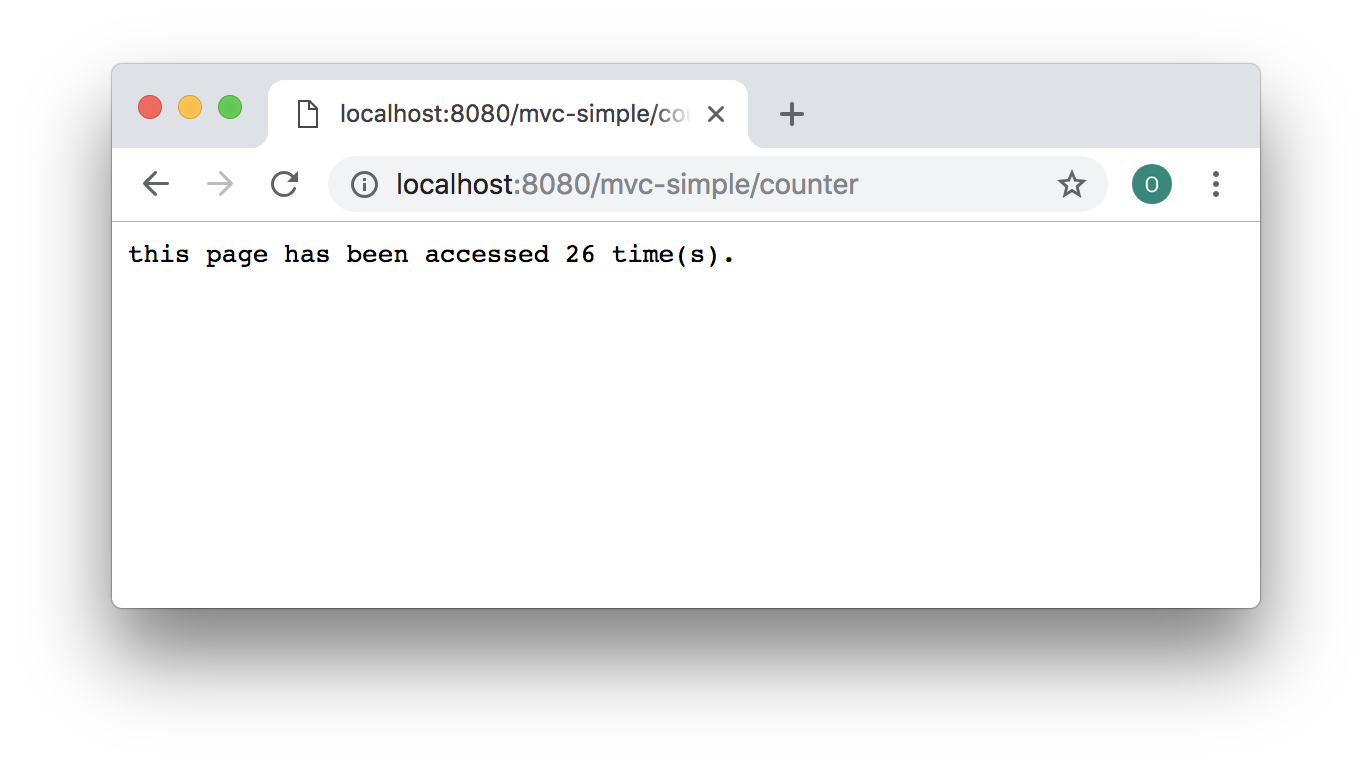
\includegraphics[width=1.0\linewidth]{Figures/screenshot-servlet-counter.png}
	\caption{The application manages an access counter shared by all users}
  \label{fig:screenshot-servlet-counter}
\end{figure}

Implementing this feature looks easy enough. Let us create an HttpServlet and define a \texttt{counter} instance variable. In the \texttt{doGet} method, simply get and increment its value and generate the response page. Let us also make it possible to reset the counter by sending a \texttt{command} parameter in the query string with the \texttt{reset} value. The code is shown in \ref{lst:counterServletWrong}.

\lstset{
	caption={Incorrect implementation of the counter servlet},
	language=java,
	label={lst:counterServletWrong}
}
\vspace{10pt}
\begin{minipage}{\linewidth}
\begin{lstlisting}[frame=single]
package ch.heigvd.amt.mvcsimple.presentation;

import ch.heigvd.amt.mvcsimple.model.Quote;

import javax.servlet.ServletException;
import javax.servlet.annotation.WebServlet;
import javax.servlet.http.HttpServlet;
import javax.servlet.http.HttpServletRequest;
import javax.servlet.http.HttpServletResponse;
import java.io.IOException;

@WebServlet(name = "CounterServlet", urlPatterns = "/counter")
public class CounterServlet extends HttpServlet {

    private int counter = 0;

    protected void doGet(HttpServletRequest request, HttpServletResponse response) throws ServletException, IOException {
        String command = request.getParameter("command");
        if ("reset".equals(command)) {
            counter = 0;
        } else {
            counter = counter + 1;
        }
        response.getWriter().println("this page has been accessed " + counter + " time(s).");
    }
}
\end{lstlisting}
\end{minipage}


\subsection{Problem: servlets are not thread-safe}

\marginpar{Using member variables in servlets is dangerous. Either they have to be thread-safe objects or the access need to be synchronized. }

At first glance, the application works as expected. When the developer deploys the application and performs manual tests in the browser, the counter seems to work perfectly. Time to release to production? Not quite: there is a serious problem with this code. When using a development platform such as Java EE, the lifecycle of objects is managed by a framework. To write correct code, it is important to study what happens and to be aware which methods are thread-safe and which are not.

The Servlet specification clearly states that it is possible for several threads to be in the \texttt{doGet} method at the same time. Therefore, it is possible to have a race condition on instance variables. The Javadoc documentation for the \texttt{HttpServlet} class states: \emph{Servlets typically run on multithreaded servers, so be aware that a servlet must handle concurrent requests and be careful to synchronize access to shared resources. Shared resources include in-memory data such as instance or class variables and external objects such as files, database connections, and network connections.}

To show that the code in Listing \ref{counterServletWrong}, let us consider a concrete scenario. Let us imagine that two browsers send a request to the servlet at the same time. As a result, the \texttt{doGet} method is executed twice, on two threads \texttt{T1} and \texttt{T2}. Let us imagine that before the scenario, the counter has a value of \texttt{100}. If the two threads reach line 22 at the same time, the following sequence of operations is possible: 

\begin{enumerate}
\item \texttt{T1} reads \texttt{counter} value (\texttt{100})
\item \texttt{T2} reads \texttt{counter} value (\texttt{100})
\item \texttt{T1} sets \texttt{counter} value to \texttt{100 + 1} (\texttt{101})
\item \texttt{T2} sets \texttt{counter} value to \texttt{100 + 1} (\texttt{101})
\end{enumerate}

This scenarios that it is possible to miss counter updates. Hence, if the servlet is accessed 1'000 times under load, it is possible that the counter has a smaller value than 1'000. How do we show that this is indeed possible? How do we create an experiment to produce the bug and have an evidence of the problem? Working with the debugger might provide some help, but we would most likely have to modify the code and introduce some statements to pause the execution of the program. Let us take a different route and create a race condition through load testing.

\subsection{Design of a test plan with JMeter}

\marginpar{A demonstration has been recorded in a webcast. It is available in the companion Youtube playlist, in a series of 4 videos entitled ``Load testing with JMeter''}

The test plan created in JMeter to produce the error condition is shown in Figure \ref{fig:screenshot-jmeter-servlet-counter-bug}. The tree view on the left contains the following elements:

\begin{itemize}
\item The \emph{setUp Thread Group} is used to send one single HTTP request at the beginning of the test procedure.
\item To do that, we configure the HTTP Request sampler to send a \texttt{GET} request to \texttt{/mvc-simple/counter?command=reset}.
\item \emph{Virtual users} is a thread group that simulates concurrent users. We set the number of threads to 20 and do 1 iteration of the plan.
\item the View Results Tree is a listener that allows us to see that last requests and responses processed by JMeter. In the screenshot, it is disabled because we have completed the test design phase and do not need it anymore.
\item In the \emph{Loop Controller}, we specify that we want every virtual user to perform 100 iterations of the scenario.
\item The scenario consists of sending an HTTP request to \texttt{/mvc-simple/counter} and to pause for a brief period (the \emph{Gaussian Random Timer} is configured with a deviation of 10 ms and delay offset of 30 ms.
\item The \emph{tearDown Thread Group} is used to issue one last HTTP request to retrieve the value of the counter at the end of the test. We use the \emph{Regular Expression Extractor} to retrieve the counter value, the Response Assertion to check if the counter value is equal to 2001 (\emph{20 virtual users * 100 iterations per virtual user + 1 last request}).
\item the \emph{Debug PostProcessor}, \emph{Assertion Results} and \emph{View Results Tree} are used to display the test results and to inspect the value of the extracted variables.
\end{itemize}

\begin{figure}[]
	\centerline{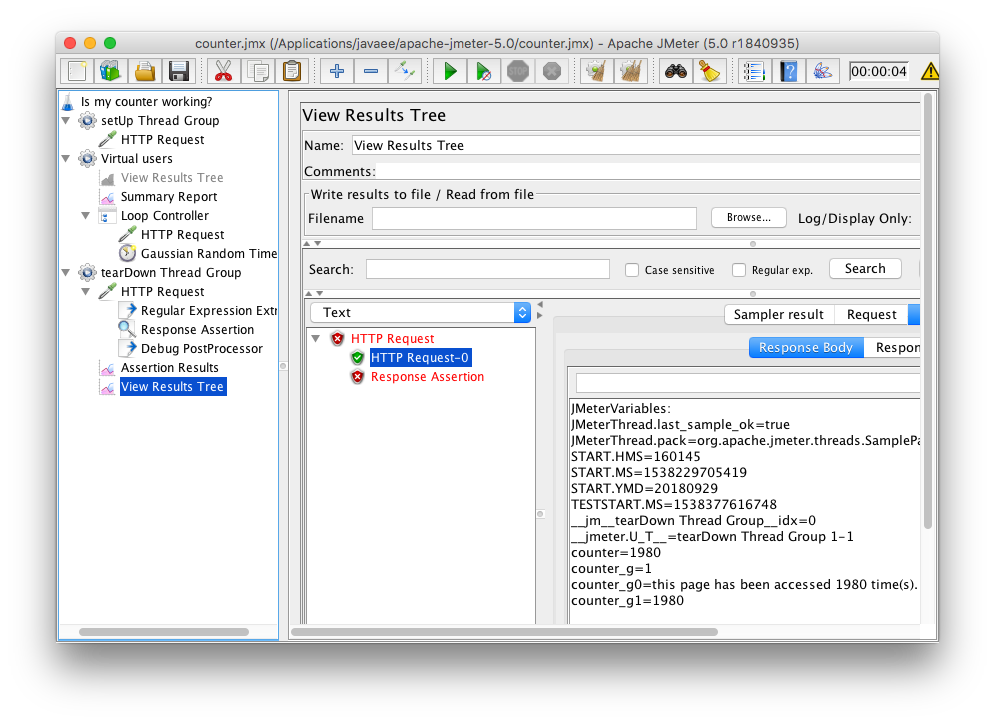
\includegraphics[width=1.3\linewidth]{Figures/screenshot-jmeter-servlet-counter-bug.png}}
	\caption{The test plan defines a complete scenario}
  \label{fig:screenshot-jmeter-servlet-counter-bug}
\end{figure}

\subsection{Interpretation of the results}

In the screenshot of the JMeter test plan, we see that the \emph{Response Assertion} is displayed in red, which indicates a problem: the expect final value for the counter is not 2001. If we click on the \emph{HTTP Request-0} node in the tree view, we see the evaluation of the regular expression and the value of the counter variable. It is equal to 1980. When running the load test multiple times, counter will generally have a different value at each run, because concurrency makes the behavior non deterministic. 

\subsection{Correction of the bug}

The \texttt{CounterServlet} class can easily be fixed, as shown in Listing \ref{lst:counterServletWrong}. The code that accesses and modifies the member variable is wrapped in a synchronized block (lines 11-13). An alternative would have been to use a thread-safe class (\texttt{AtomicInteger}) instead of the int primitive type for the counter variable.

\lstset{
	caption={The counter servlet modified to deal with concurrent requests},
	language=java,
	label={lst:counterServletWrong}
}
\vspace{10pt}
\begin{minipage}{\linewidth}
\begin{lstlisting}[frame=single]
@WebServlet(name = "CounterServlet", urlPatterns = "/counter")
public class CounterServlet extends HttpServlet {

    private int counter = 0;

    protected void doGet(HttpServletRequest request, HttpServletResponse response) throws ServletException, IOException {
        String command = request.getParameter("command");
        if ("reset".equals(command)) {
            counter = 0;
        } else {
            synchronized (this) {
                counter = counter + 1;
            }
        }
        response.getWriter().println("this page has been accessed " + counter + " time(s).");
    }
}
\end{lstlisting}
\end{minipage}

\section{Case study: HTTP sessions and scalability}

While HTTP is a stateless protocol, many web applications built on top of the protocol have a notion of session. Think about applications with \emph{login} and \emph{logout} features. Think about a typical e-commerce site with a \emph{shopping cart}. In these applications, there is a state associated with every session and it needs to be stored somewhere. As a matter of fact, there are quite a few places to store it and the choice can have a dramatic impact on performance, scalability and availability. There is no single best practice and trends have evolved over the years.

When Java EE appeared on the market, the most common practice was to avoid storing session state in the database. The reason was that the database was usually on a remote host. At the time, networks were slower and even if the application host and database host were on the same internal network, remote calls were slow. Memory was also expensive, which means that databases were not able to store large data sets in memory caches. For these reasons, it made sense to store conversation state in the presentation tier.

The servlet API makes this very easy, thanks to the \texttt{HttpSession} class. When implementing the \texttt{doGet} method, the developer can obtain a HttpSession from the request parameter. He can then store arbitrary object graphs by calling \texttt{session.setAttribute("name", value)}. The great thing about this API is that it is very easy to use. The terrible thing about it is that it is very easy to use and that inexperienced developers sometimes do not realize the implications of making these calls. Obviously, storing an object in the session consumes memory. This memory remains allocated as long as the session is active. There are two main reasons for the session to become inactive. Sometimes, the developer can explicitly call \texttt{session.invalidate()} when he knows that the user has finished his session (e.g. he has clicked on a \emph{logout} button). However, users often just stop interacting with the web application and it is impossible to know for sure that they are done. Application servers can be configured with a maximum session idle period: if no request is received from a user within this period, then the session is terminated and the resources are reclaimed. Setting the maximum session idle time to 5 minutes, 30 minutes or 3 hours can make a huge difference on a high-traffic web application.

Another factor to consider is the \ac{JVM} configuration parameters for the application server. When using a Java EE application server in development, one often goes with the default parameters. This includes memory settings, such as the maximum heap size. In production, it is usually necessary to increase the default value. By how much? If you know how many active sessions should be supported by a node and if you know how much memory is consumed by the session state, then you can estimate the memory requirements for this aspect of the application. Of course, while this is something that you can model and calculate, it is also something that you should measure through experiments. As you can imagine, this is where a tool like JMeter is very helpful.

\emph{[TODO: document test procedure with JMeter]}


\section{Case study: performance impact of pagination}

\emph{[TODO]}

\section{Case study: performance impact of caching}

\emph{[TODO]}

\section{Case study: performance impact of ORM tuning}

\emph{[TODO]}


\section{Questions}

To answer these questions, you will need to have read the chapter but also to have done some research. Make sure that you are able to answer every question. Discuss your responses with your peers.

\emph{[TODO]}



